\chapter{Estrategia de control}
% ----------------------

\label{C:Formas de control}

\section{Principio de estrategia de control.}
El algoritmo PID (proporcional, integral, derivado) está formado por la suma de tres componentes, Proporcional, Integral y Derivativo) Matemáticamente, un controlador PID tiene la siguiente formulación: \par
\begin{equation}
Output(t)=K_p\cdot e(t)+K_i\int_0^t e(t)\cdot dt+K_d\cdot \frac{de}{dt}
\end{equation} \par 
Cada componente del PID es \entreComillas{independiente} de las demás. en el sentido de que cada uno calcula una salida de lo que \entreComillas{para él} debería hacer para obtener la respuesta adecuada. \par 
Los tres componentes se suman para dar la salida del controlador. Cada uno cumple una cierta función y mejoran cierta parte de la respuesta. Y cuando los tres componentes trabajan juntos, en la proporción adecuada, consiguen un gran comportamiento. \par 
Cada componente tiene un parámetro $K_p$, $K_i$ y $K_d$, respectivamente. Estos parámetros indican la ponderación que tiene en el resultado final.
\begin{itemize}
\item El componente proporcional reacciona al presente.
\item El componente integral reacciona al pasado, y aporta “memoria” al controlador.
\item El componente derivado reacciona al futuro, y aporta “predicción” al controlador.
\end{itemize} \par 
Resumiendo los efectos del PID:
\begin{itemize}
\item Componente proporcional:
\begin{itemize}
\item Valor bajo de $K_p$, respuesta lenta.
\item Valor alto de $K_p$, sobrepaso, oscilación, e incluso inestabilidad.
\item No consigue eliminar el error en régimen estacionario.
\end{itemize}
\item Integral:
\begin{itemize}
\item Elimina el error estacionario.
\item Demasiado $K_i$, oscilación e inestabilidad.
\end{itemize}
\item Derivativo:
\begin{itemize}
\item Mejora el comportamiento general
\item Demasiado $K_d$, comportamiento indeseado en la salida.
\item Muy sensible al ruido.
\item Muy sensible a cambios bruscos en el error (perturbaciones o cambios de consigna)
\end{itemize}
\end{itemize}\par 

En base a estos conceptos, se propone el siguiente esquema de control presentado en la Figura \ref{F:Esquema_Control}. En el mismo, los parámetros configurables por el usuario serán la tensión de referencia, la corriente máxima de control y un valor de corriente de cortocircuito que desconectaría la carga por seguridad. \par 
La corriente máxima de control $I_{cc}$ será el valor utilizado por el algoritmo anti-windup que se explicará en las secciones porvenir. Esta provoca que la acción de control resultante del lazo de tensión externo sea menor a este valor introducido por el usuario, de modo que durante la operación normal no se exceda este valor de corriente incluso si para ello es necesario bajar el nivel de tensión a la salida. \par 
Por otro lado, la variable $I_{max}$ es el valor al cual se ajustará el potenciómetro digital, cuya función es establecer un valor de referencia al comparador analógico, donde si la tensión proporcional a la corriente actual es mayor a este, se abre forzosamente la llave que excita al relé y se genera una interrupción en el microcontrolador. Esto se aplica como medida adicional de protección, resultando en una respuesta más rápida dado que no depende del lazo de control para desconectar la carga.\par 

\begin{figure} [H]
	\centering
	\includegraphics[width=\textwidth]{./imagenes/Esquema_Control.jpg}
	\caption{Diagrama de bloques del funcionamiento del controlador.}
	\label{F:Esquema_Control}
\end{figure} \par 
Tanto para el lazo interno de corriente como para el lazo externo de tensión se utilizará un controlador PID. El controlador del lazo de tensión le brindará la corriente de referencia a seguir al lazo de corriente, cuya salida del controlador será el voltaje a aplicar sobre la base del transistor del regulador lineal con BJTs. \par 

La ecuación de un controlador PID en tiempo continuo está dada por: \cite{BotteronSC1}
\begin{equation}
u(t)=K_pe(t)+K_i\int _0^t e(t)dt +K_d\frac{de(t)}{dt}
\end{equation} \par 
Siendo su expresión en el dominio de Laplace:
\begin{equation}
U(s)=(K_p+\frac{K_i}{s}+sK_d)E(s)
\end{equation}\par 
Donde considerando una aproximación rectangular \textit{backward}, la acción de control resultante en función de la variable 'z' resulta:
\begin{equation}
s\approx\frac{(z-1)}{zT} \quad \to \quad U(z)=[K_p+K_iT\frac{z}{z-1}+\frac{K_d}{T}\frac{(z-1)}{z}]E(z)
\end{equation}\par 
Aplicando la anti-transformada $Z$ a $U(z)$ se obtiene la ecuación a diferencias finitas ya conocida:
\begin{equation}
u(k)=K_pe(k)+K_iT\sum_{n=1}^k e(n)+\frac{K_d}{T}[e(k)-e(k-1)]
\end{equation}\par 
Esta expresión de la acción de control depende del error actual $e(k)$, donde no considera el atraso de implementación digital $T_d$. \par 
Por ello se introduce una predicción del error:
\begin{equation}
e(k)=e(k-1)+[e(k-1)-e(k-2)]
\end{equation}\par 
De esta forma la acción de control depende de los errores anteriores y $u(k)$ no se ve afectada por el atraso de implementación digital, pudiendo compensar eficientemente las perturbaciones. \par 
Por lo tanto, la ecuación a diferencias de la acción de control resulta:
\begin{equation} \label{eq:PIDp}
u_{PIDp}(k)=u_{PIDp}(k-1)+K_1e(k-1)+K_2e(k-2)+K_3e(k-3)
\end{equation}\par 


\section{Lazo de corriente}
Para realizar el diseño del lazo de control interno es necesario realizar un modelado del mismo. Al utilizar diversos softwares de simulación (PSIM y TINA TI), se verificó que efectivamente, mientras se encuentre en la zona lineal los transistores, la corriente de salida dependerá linealmente de la tensión de entrada, $I_L=k\cdot V_{ctrl}$\par 
Sin embargo, determinar el valor de k no es sencillo, dado que en los extremos de la recta de carga, el sistema se vuelve no lineal como se observa en la \ref{F:Recta_de_carga_corriente}. Además. existe un cierto valor mínimo en el cual el transistor se mantendrá en corte (aproximadamente $V_B=0,3V$). Por ende, se asumirá una planta con ganancia unitaria mientras que se retocarán las ganancias del controlador experimentalmente hasta alcanzar la respuesta deseada.\par 
\begin{figure} [H]
	\centering
	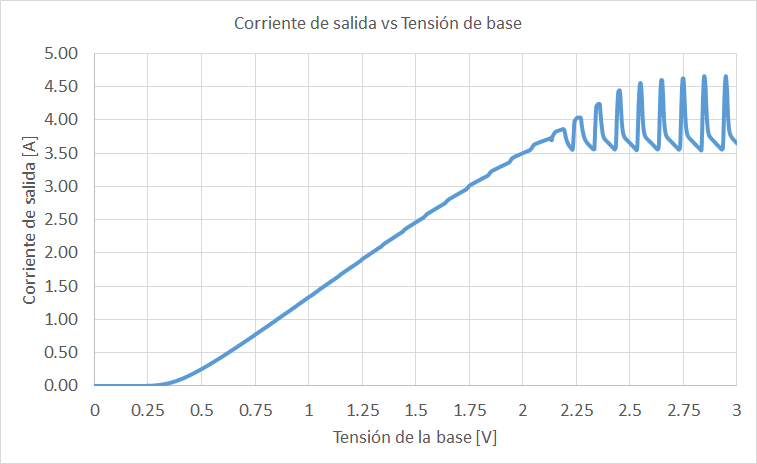
\includegraphics[width=0.8\textwidth]{./imagenes/Recta_de_carga_corriente.png}
	\caption{Corriente de salida vs tensión de base para condición de plena carga ($R=10\Omega$).}
	\label{F:Recta_de_carga_corriente}
\end{figure} \par 

Para determinar el controlador a utilizar, recordamos que un lazo cerrado presenta la siguiente expresión:
\begin{equation}
G_{LC}(z)=\frac{G_P(z)\cdot G_C(z)}{1+G_P(z)\cdot G_C(z)}
\end{equation}
Donde $G_P(z)$ será una constante igual a 1 para este caso, mientras que  $G_C(z)$ será un controlador PID:
\begin{equation} 
\begin{split}
G_{C_{PID}}(z)&=K_P+K_IT\frac{z}{z-1}+\frac{K_D}{T}\frac{z-1}{z} \\
G_{C_{PID}}(z)&=\frac{K_pz^2+K_iz+K_d}{z^2-z}
\end{split}
\end{equation}\par 

Determinamos la ubicación de los polos deseados en función de las siguientes especificaciones: un $5\%$ de sobrepaso y un tiempo de asentamiento de $0,1s$. Esto resulta en los polos $s_{1,2}=-40\pm 41,95i$ del plano 's'. Para llevarlos al plano 'z' se aplica $z=e^{sT}$, obteniendo $z_{1,2}=0,8999\pm 0,0947i$. Al tercer polo del controlador PID lo ubicamos cerca del origen para no afectar significativamente la respuesta del sistema $z_3=0,1$.\par 
Queremos que los polos del lazo cerrado coincidan con $z_1$, $z_2$ y $z_3$. La ecuación característica del sistema en lazo cerrado es:
\begin{equation}
(z-z_1)(z-z_2)(z-z_3)=z^3-(z_1+z_2+z_3)z^2+(z_1z_2+z_1z_3+z_2z_3)z-z_1z_2z_3
\end{equation}
Donde $A=z_1+z_2+z_3$, $B=z_1z_2+z_1z_3+z_2z_3$ y $C=z_1z_2z_3$. Las ecuaciones a resolver son:
\begin{equation}
G_P(K_pz^2+K_iz+K_d)=(z-1)(z^2-Az+Bz-C)
\end{equation}
De las ecuaciones características $K_p=A-1$, $K_i=B$ y $K_d=C$, por lo que $K_p=0,8997$, $K_i=0,9987$ y $K_d=0,0819$. En la Figura  \ref{F:Resp_lazo_corriente} se presenta la respuesta al escalón del lazo de corriente diseñado.
\begin{figure} [H]
	\centering
	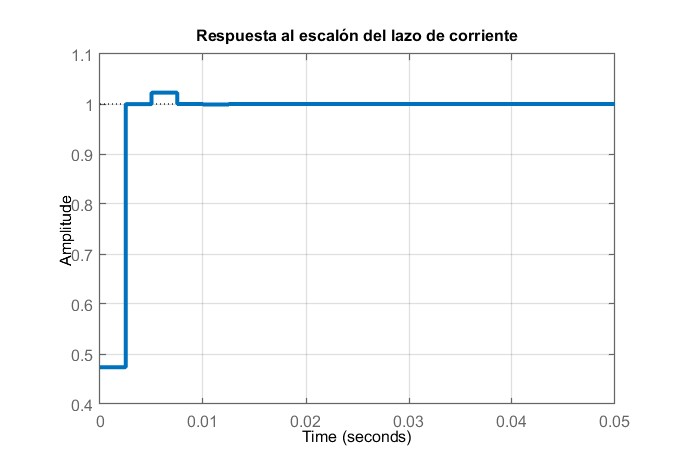
\includegraphics[width=0.8\textwidth]{./imagenes/Resp_lazo_corriente.jpg}
	\caption{Respuesta al escalón del lazo interno de corriente diseñado.}
	\label{F:Resp_lazo_corriente}
\end{figure} \par 
Se puede observar que el sistema responde rápidamente, con un pequeño sobrepaso cumpliendo las especificaciones iniciales. También logra reducir el error a cero, siguiendo el valor de la referencia en régimen permanente. \par 

\section{Lazo de tensión}
Para realizar el diseño del lazo de control externo de tensión se modela la carga de salida, obteniendo la función de transferencia que vincule la tensión de salida con su corriente. \par 
Suponiendo una carga Resistiva-Capacitiva (RC) de $C=470\mu F$ y $R=10\Omega$. Por Laplace se establecen las siguientes relaciones:\par 
\underline{Resistencia}:
\begin{equation}
v(t)=i(t)R \Leftrightarrow V(s)=I(s)R
\end{equation}\par 
\underline{Capacitor}:
\begin{equation}
v(t)=\frac{1}{C}\int i(t)dt \Leftrightarrow V(s)=\frac{1}{sC}I(s)+\frac{1}{s}v(0)
\end{equation}

\begin{figure} [H]
	\centering
	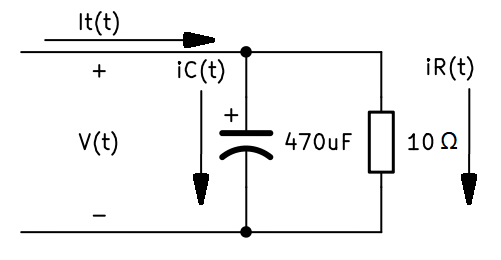
\includegraphics[scale=0.6]{./imagenes/CircuitoRC.png}
	\caption{Modelo de la salida de tensión.}
	\label{F:CircuitoRC}
\end{figure} \par 
Aplicando la ley de Kirchoff para los nodos:
\begin{equation}
i_t(t)=i_R(t)+i_C(t)
\end{equation}\par 
Pasando al dominio de Laplace:
\begin{equation}
I_t(s)=I_R(s)+I_C(s)
\end{equation}\par 
Reemplazando por lo obtenido anteriormente:
\begin{equation}
I_t(s)=\frac{V(s)}{R}+sCV(s)
\end{equation}\par 
Finalmente obtenemos el modelo que define la carga:
\begin{equation}
G_P(s)=\frac{V(s)}{I_t(s)}=\frac{1}{\frac{1}{R}+sC}
\end{equation}\par 
Tomando la expresión de $G_P(s)$ y llevándola al dominio discreto, en conjunto con el lazo cerrado de corriente obtenido en la sección anterior es posible diseñar el control externo de tensión de forma tal que cumpla con ciertas especificaciones de diseño. Para el diseño se considera la planta en una condición de vacío, siendo el valor del capacitor de salida $C=470\mu F$ y la resistencia de carga $R=2700\Omega$. \par 
Se utiliza la técnica de reubicación de polos por lugar geométrico de las raíces para obtener las constantes del controlador. Planteando inicialmente un PI predictivo con las siguientes características: un sobrepaso del $5\%$ y un tiempo de asentamiento de $0,5s$. El controlador obtenido por este método es el que se muestra a continuación:
\begin{equation}
G_{Cv}(z)=K\frac{(z-a)}{z(z-1)}=\frac{0,006965 z - 0,006819}{z^2 - z}
\end{equation} \par 
Adicionalmente, se agregan otros dos controladores obtenidos de forma iterativa con la planta real para su comparación:
\begin{equation}
G_{Cv_{v2}}=\frac{0,011 z^2 - 0,0102 z + 1\cdot 10^{-5}}{z^3 - z^2}
\end{equation}
\begin{equation}
G_{Cv_{v3}}=\frac{0,012 z^2 - 0,012 z + 1\cdot 10^{-5}}{z^3 - z^2}
\end{equation}\par 
Se presenta a continuación en la Figura \ref{F:Resp_lazo_tension_vacio} la comparación de las respuestas al escalón del lazo externo de tensión para los distintos controladores presentados, por un lado, el PI obtenido por la reubicación de polos a partir del lugar geométrico de las raíces, frente a los dos controladores obtenidos de forma iterativa.
\begin{figure} [H]
	\centering
	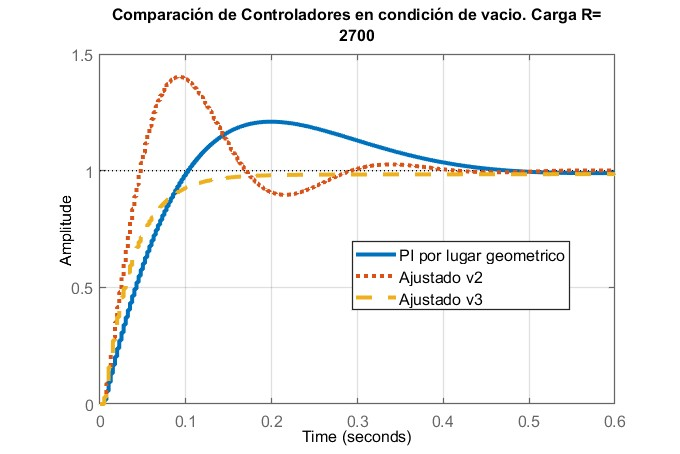
\includegraphics[width=0.8\textwidth]{./imagenes/Resp_lazo_tension_vacio.jpg}
	\caption{Comparación de las respuestas al escalón del lazo externo de tensión diseñado frente a los ajustados propiamente para la condición de vacío $R=2700\Omega$.}
	\label{F:Resp_lazo_tension_vacio}
\end{figure} \par 
Se puede observar que el controlador PI diseñado no cumple con la especificación del sobrepaso para la condición de vacío, mientras que $G_{Cv_{v2}}$ presenta mayor sobrepaso y oscilación y finalmente $G_{Cv_{v3}}$ logra una respuesta sobreamortiguada, siendo la mejor opción para esta condición de vacío.\par 
A continuación, se toman estos controladores y se los aplica en una condición de carga con $R=10\Omega$, los resultados se presentan en la Figura \ref{F:Resp_lazo_tension_carga}.
\begin{figure} [H]
	\centering
	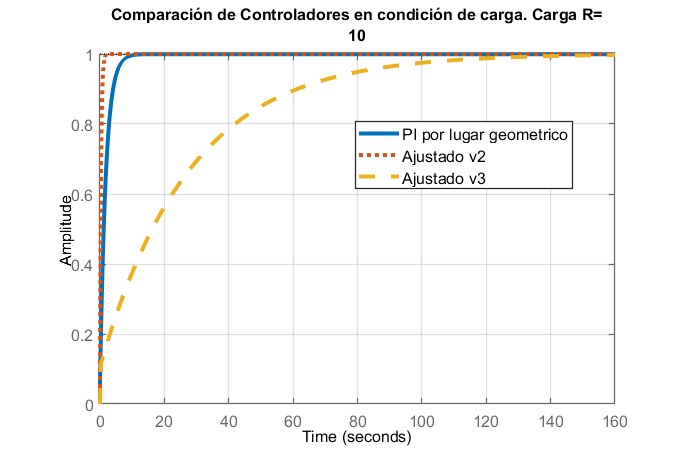
\includegraphics[width=0.8\textwidth]{./imagenes/Resp_lazo_tension_carga.jpg}
	\caption{Comparación de las respuestas al escalón del lazo externo de tensión ante una condición de carga $R=10\Omega$.}
	\label{F:Resp_lazo_tension_carga}
\end{figure} \par 
Podemos observar que en este caso, la respuesta del sistema se vuelve muy lenta, siendo el controlador que mejor desempeño presenta el $G_{Cv_{v2}}$. Por lo que se puede concluir que existe una relación de compromiso entre el desempeño del sistema ante distintas condiciones de carga. \par

\section{Algoritmo Anti-Windup}
La acción de control resultante, ya sea $u_v(k)$ o $u_i(k)$, puede ser saturada o limitada a valores positivos y/o negativos en casos en los que se presentan sobretensiones o sobrecorrientes por encima de los valores permitidos. La limitación de la acción de control a un valor fijo, significa que el sistema pierde la controlabilidad de los estados del proceso dado que sería similar a imponer un valor de referencia fijo; en este caso, esta referencia sería la del lazo interno de control de corriente. Esta situación provoca que el error entre la referencia y la salida varíe, tanto en sentido positivo como negativo, sin poder llevarlo a cero y por ende, al existir una acción de integración que acumula a cada periodo de muestreo, la misma puede crecer sin control, limitada únicamente por el tamaño de los registros que almacenen esta variable, con una excursión entre un valor máximo positivo a un valor máximo negativo, pasando el sistema lineal, a ser no lineal. Si esta situación no es controlada, puede provocar un comportamiento oscilatorio de los estados del proceso y si por acaso la acción de control vuelve a situarse dentro de los valores normales, puede que no vuelva a operar correctamente y deba reiniciarse el proceso. Este aumento sin control de la acción integral es lo que se denomina \textit{windup}, y es por lo que debe implementarse una acción \textit{anti-windup}. \par
Se opta por utilizar una forma simple de \textit{anti-windup} que consiste en que la integración del controlador dada por $u[(k-1)T_s]$ sea actualizada según el valor de saturación y los valores de los errores actual y anteriores, afectados por sus coeficientes. Esto provoca que a cada periodo de muestreo y mientras se mantenga limitada la acción de control, el error de tensión $e_v(kTs)$ se mantenga acotado y por ende también las variables de estados del proceso.
Matemáticamente, el algoritmo se representa de la siguiente manera:
\begin{itemize}
\item Condición 1: Valor mayor al valor de limitación positivo: \\
Si $u(kT_s)\geq u_{sat}$
\begin{equation}
	u[(k-1)T_s]=u_{sat}-K_{1}\cdot e(kT_s)-K_{2}\cdot e[(k-1)T_s]-K_{3}\cdot e[(k-2)T_s]
\end{equation}

\item Condición 2: Valor menor al valor de limitación negativo. \\
Si $u(kT_s)\leq -u_{sat}$
\begin{equation}
	u[(k-1)T_s]=-u_{sat}-K_{1}\cdot e(kT_s)-K_{2}\cdot e[(k-1)T_s]-K_{3}\cdot e[(k-2)T_s]
\end{equation}
\item Condición 3: Valor dentro de la región lineal \\
Si $u_{sat}>u(kT_s)>-u_{sat}$
\begin{equation}
	u[(k-1)T_s]=u(kT_s)
\end{equation}
\end{itemize} \par 

Además, a cada periodo de muestreo, ya sea que la acción de control resulte limitada o no, debe actualizarse el error de tensión, o sea:
\begin{equation}
	e[(k-2)T_s]=e[(k-1)T_s] \qquad	e[(k-1)T_s]=e(kT_s)
\end{equation}

\section{Modos de operación de la fuente.}
En base a las simulaciónes, cálculos y estrategias de control se plantearon los tres modos de funcionamiento disponibles para adaptarse a las diversas necesidades de aplicación. A continuación, se describen brevemente los principales modos de operación que estarán disponibles en el menú, su principio de funcionamiento, y qué parámetros serán configurables. \par 
\subsection{Modo Tensión}
En este modo, la fuente de alimentación establece inicialmente el valor máximo de tensión deseado. Posteriormente, limita la corriente máxima de umbral que la carga podrá obtener. Este modo es especialmente útil cuando se requiere controlar la tensión suministrada a la carga de manera precisa y garantizar la seguridad del sistema al limitar la corriente máxima.\par
Para lograr este control se utiliza el lazo completo de la Figura \ref{F:Esquema_Control} encerrado en violeta, en donde el mismo consta de un lazo interno de corriente y uno externo de tensión con ambas referencias externas de valores constantes. \par

\subsection{Modo Corriente}
En el modo de corriente, la fuente de alimentación establece y controla la corriente suministrada a la carga. Este modo es útil en situaciones donde es crítico mantener la corriente dentro de ciertos límites para proteger los componentes de la carga y garantizar su correcto funcionamiento.\par 
Aquí solamente corresponde utilizar una parte interna del lazo de control que corresponde a la zona encerrada en rojo de la Figura \ref{F:Esquema_Control} que es el que se vincula con la corriente, de modo que la cantidad de operaciones necesarias para definir la acción de control será menor y mejora gradualmente la velocidad de actualización de la acción de control. \par

\subsection{Modo Rampa}
El modo de rampa tiene como objetivo generar un aumento gradual y lineal de la tensión suministrada a la carga durante un período de tiempo determinado. Los parámetros configurables en este modo incluyen la tensión final deseada para la carga y el tiempo en el cual se alcanzará esta tensión desde un valor inicial de 0V. Este modo es útil en aplicaciones donde se requiere un inicio suave del sistema para evitar sobrecargas o picos de corriente al iniciar la energización de componentes. Especialmente útil en cargas como lo podrían ser por ejemplo motores.\par 
Para la implementación del mismo, como para el modo de tensión, corresponde utilizar el lazo de control completo que engloba tensión y corriente. La diferencia unicamente radicará en que si bien la corriente máxima limitante se mantendrá fija, la tensión de referencia verá un aumento gradual escalonado en base al tiempo o duración de la rampa configurado. \par
